% Created 2021-05-10 Mon 20:02
% Intended LaTeX compiler: pdflatex
\documentclass[11pt]{article}
\usepackage[utf8]{inputenc}
\usepackage[T1]{fontenc}
\usepackage{graphicx}
\usepackage{grffile}
\usepackage{longtable}
\usepackage{wrapfig}
\usepackage{rotating}
\usepackage[normalem]{ulem}
\usepackage{amsmath}
\usepackage{textcomp}
\usepackage{amssymb}
\usepackage{capt-of}
\usepackage{hyperref}
\usepackage{listingsutf8}
\usepackage{minted}
\usepackage{arxiv}
\author{Marco Hassan}
\date{\today}
\title{}
\hypersetup{
 pdfauthor={Marco Hassan},
 pdftitle={},
 pdfkeywords={},
 pdfsubject={},
 pdfcreator={Emacs 27.2.50 (Org mode 9.4.4)}, 
 pdflang={English}}
\begin{document}

\newtheorem{theorem}{Theorem}

\title{Parameter Learning in Bayesian Networks under Uncertain Evidence  \textendash  \ An Exploratory Research.}
\author{
  Marco Hassan 	           	\\
  Zurich, CH		\\
  \\
  \\
  Master Thesis \\
  Presented to the Eidgenossische Teschnische Hochschule Zurich \\
  In Fulfillment Of the Requirements for \\ 
  the Master of Science in Statistics \\
  \\
  Supervisor: PhD. Radu Marinescu \\
  Co-Supervisor: Dr. Markus Kalisch \\
  %% examples of more authors
  %% \AND
  %% Coauthor \\
  %% Affiliation \\
  %% Address \\
  %% \texttt{email} \\   
  %% \And
  %% Coauthor \\
  %% Affiliation \\
  %% Address \\
  %% \texttt{email} \\
  %% \And
  %% Coauthor \\
  %% Affiliation \\
  %% Address \\
  %% \texttt{email} \\
}

\begin{article}

\maketitle

\newpage

\tableofcontents

\newpage

\listoffigures
\listofalgorithms
\listoftables

\newpage

\section{{\bfseries\sffamily TODO} Bayesian Networks Overview and Definition \& Literature Review}
\label{sec:org288d2b2}


\section{{\bfseries\sffamily TODO} Learning under Complete Evidence}
\label{complete-learning}
As vastly documented in the literature there are essentially two
types of approaches when performing the task of parameter
learning. The first one is a parameter estimation via \emph{Maximum
Likelihood Estimation (MLE)} as in \cite{Myung_2003} while the second
amounts to parameter estimation via \emph{Bayesian Learning} as presented
in \cite{Smith_2001}.


\subsection{{\bfseries\sffamily TODO} write the gloabl decomposition etc. properties}
\label{sec:orga601665}


\section{Types of Uncertain Evidence}
\label{sec:org6311014}

So far we discussed the case of parameter learning in Bayesian
Networks in the case of complete evidence, i.e. in the case we could
observe a realization for each random variable in the network.

As we discussed, in such a case important properties hold for the
network such as the global likelihood decomposition. This allows the
possibility to work with local conditional probabilities in order to
reach the optimal solution.

One more interesting case is the one treated by \cite{Mrad_2015},
\cite{Wasserkrug_all}. The argument posed by the authors is that under
many settings complete evidence is not possible.

In many cases there might be a hiding mechanism active that might
hide some of the realizations. Think for instance at a
malfunctioning sensor that sporadically measures input. Or think for
instance at medical settings where different patients might be
measured different variables.

Albeit the case of missing evidence greatly alters the way through
which it is possible to learn the parameters of the network, there
are multiple possible solutions to get to the results - see for
instance \cite{koller2009probabilistic}.

A more interesting case is posed by \emph{uncertain evidence} as
introduced by \cite{Mrad_2015}. The authors distinguish three types of
non-complete evidence:

\begin{itemize}
\item likelihood evidence

\item fixed probabilistic evidence

\item non-fixed probabilistic evidence
\end{itemize}

We will use throughout this document the definition as in
\cite{Mrad_2015} which we will briefly summarize next.

\begin{definition}
Hard evidence: A finding on a variable commonly refers to an
instantiation of the variable. This can be represented by a vector
with one element equal to 1, corresponding to the state the variable
is in, and all other elements equal to zero. This type of evidence
is usually referred to as hard evidence.
\end{definition}

\\\\

\begin{definition}
Uncertain evidence: evidence that cannot be represented by a vector
as in the hard evidence case.
\end{definition}

\\\\

\begin{definition}
Likelihood evidence: in such type of evidence there is uncertainty
about the veracity of an observation, such as, for example, the
information given by an imperfect sensor. Such uncertainty is
expressed in terms of relative likelihood of observing one
realization vis à vis another one. 
\end{definition}

\\\\

\begin{definition}
Probabilistic evidence: we talk about probabilistic evidence when we
have a set of probabilistic finding on multiple random variables X in the network
specified by a local probability distribution R(X).
\end{definition}  

Notice that a probabilistic finding R(X) on a variable X of a
Bayesian network replaces any prior belief or knowledge on X. As a
consequence, the prior P (X) is not used in the propagation of R(X),
and any previous finding or belief on X is lost.

Notice moreover the following distinction between \emph{fixed} and
\emph{non-fixed} probabilistic evidence:

\begin{definition}
Fixed (Non-fixed) Probabilistic evidence: A probabilistic finding
is fixed (non-fixed) when the distribution R(X) can not be (can
be) modified by the propagation of other findings.
\end{definition}  

Such that it is all about how the \emph{arrival of evidence} as in the
following schema from \cite{Mrad_2015} can update the cognitive state:

\begin{figure}[htbp]
\centering
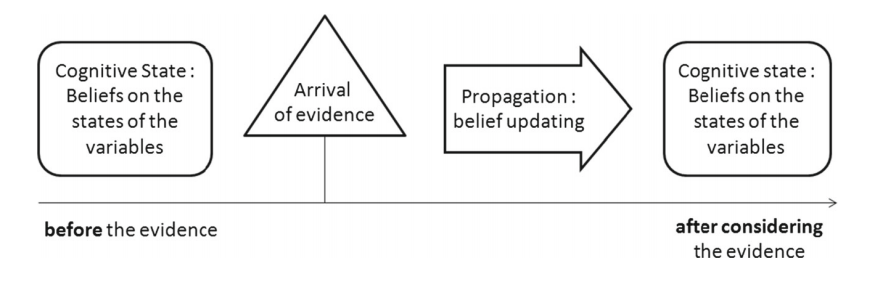
\includegraphics[width=5.0in]{/Users/marcohassan/Desktop/Bayesian_Net_Thesis/images/inference_loop.png}
\caption{Inference Loop as in Mrad et all.}
\end{figure}


Summarizing, in simple terms, we differentiate the following three
cases for the above:

\begin{enumerate}
\item In fixed-evidence we specify a probabilistic evidence \emph{all things
considered}. This means that even after new evidence is observed
on any other random variable in the network, we do not update the
cognitive state specified by the fixed probabilistic evidence.

\item In non-fixed probabilistic evidence we consider the current
structure of the tree such for the current state of the network
our conditional probability distribution is specified by the
passed probabilistic evidence. Further in-coming evidence that
will alter the network probabilistic structure will affect the
cognitive state of the current node.

\item In likelihood evidence we do not consider any prior
information. I.e. we simply specify a local likelihood ratio for
a particular evidence and we still have to run the inference step
for the current state to get the final cognitive state. I.e. as
mentioned by \cite{Mrad_2015} in contrast to probabilistic evidence
which remains unchanged by updating the observed variables,
likelihood evidence has to be combined with previous beliefs in
order to update the belief in the observed variable(s).
\end{enumerate}

We will discuss next how to handle the three types of uncertain
evidence. We will start with a discussion of missing evidence as
expanding on this it will be possible to accomplish the task
parameter learning under uncertain evidence settings.


\section{On Missing Evidence}
\label{sec:org636ff9d}

In the case of missing evidence we have two types of findings for
the random variables in our network \(<\mathscr{G}, \mathscr{X}>\).

Say that you have \(m = 1, ..., M\) instances of your network. Then on
the one hand you will have observed random variables realizations
\(d[m]\) for a subset of variables \(\mathscr{Y} \subset
  \mathscr{X}\). On the other hand you will have missing or
non-observed findings \(h[m]\) for a subset of variables
\(\mathscr{X} - \mathscr{Y}\).

As both of the parameter learning techniques, as presented in
\ref{complete-learning}, involve a likelihood term, the question is on
the way such likelihood term can be represented in the case of
missing evidence.

\subsection{{\bfseries\sffamily TODO} write down the idea of nasty likelihood and why you need the EM algorithm as a solution}
\label{sec:orgb0c0ec5}

One solution that was proposed is the one of completely ignoring
the missing evidence and computing a likelihood function just based
on the observed \(d[m]\). As argued in \cite{koller2009probabilistic},
in the case when there is no relation between the missing data and
the observed data, i.e. in the case of data \emph{missing completely at
random}, the likelihood decomposes into local probabilities so that
you can focus on terms involving your parameters of interest and
you can obtain them by standard MLE arguments as you can ignore
parameters governing missing evidence all together.

Another case is the one of data \emph{missing at random}. Here the
realization is that data \emph{missing completely at random} is a
sufficient but not necessary condition for the decomposition of the
likelihood function. I.e. in the case of conditional independence
structure the same decomposability property applies.

Then in such a case you have this likelihood just depending on
\(\sum_m P(d[m], h[m])\) such that you can ultimately use such a
likelihood by marginalizing the missing finding out. This is in
fact the approach of the EM-algorithm, which we will discuss next.


\subsection{The Mathematics of the EM}
\label{math_em}
As discussed by \cite{koller2009probabilistic} it is possible to frame
the EM as a coordinate ascent optimization of an energy function we
will define next. Given such perspective we will be able to prove the
following theorem

\begin{theorem}\label{thm:one}
Write here formally that the likelihood improves at each iteration step
\end{theorem}

Consider the following energy function:

\begin{equation} \label{eq:energy_functional}
F[P(X), Q] = E_Q[log (\tilde{P}(X))] + H_Q (X)
\end{equation}

Where \(\tilde{P}\) is an unnormalized state probability \(P =
   \frac{\tilde{P}}{Z}\) and \(H_Q\) is the entropy of the observed
particles. 

Using such energy functional \ref{eq:energy_functional} it is possible
to re-express the logarithm of the normalizing constant \(Z\) as
follows:

\begin{equation} \label{eq:energy_refurmolation}
log (Z) = F[P, Q] + D (Q||P)
\end{equation}  

where \(D(Q||P)\) is the Kullback–Leibler divergence, or relative
entropy.

We will choose next the following distribution for the particle
distribution:

\begin{equation} \label{eq:particle_distribution}
P (H | D, \theta) =   \frac{P (H, D| \theta)}{P (D| \theta)}
\end{equation}

With this choice it becomes clear that \(Z (\theta) = P (D|
   \theta)\) and \(\tilde{P} = P (H, Do| \theta)\). It
follows then immediately that given such probability function we
can compute the likelihood of realizations \(\mathscr{D}, \mathscr{H}\):

\begin{align} \label{eq:likelihood_particle}
\mathscr{L} (\theta: \mathscr{D}, \mathscr{H}) =& \  P (\mathscr{H}, \mathscr{D}| \theta)\\
\mathscr{L} (\theta: \mathscr{D}) =& \ P (\mathscr{D}| \theta)
\end{align}

where \(\mathscr{D}\) represents the observed evidence and
\(\mathscr{H}\) the missing evidence.

Such that using \ref{eq:energy_refurmolation} we can get to the
log-likelihood of the observed data in the following way:

\begin{align} \label{eq:likelihood_energy_functional_relation}
l (\theta: \mathscr{D}) =& \  F_D[\theta, Q] + D (Q (\mathscr{H}) || P (\mathscr{H}| \theta, \mathscr{D})) \\
l (\theta: \mathscr{D}) =& \  E_Q[l (\theta: \mathscr{D}, \mathscr{H})]+ H_Q (\mathscr {H}) + D (Q (\mathscr{H}) || P (\mathscr{H}| \theta, \mathscr{D}))
\end{align}

The above are two fundamental equations. It is in fact
straightforward to see that as both the relative entropy as well as
the entropy are non-negative the log-likelihood on the left hand
side above is an upper bound for the energy functional and the expected
log-likelihood relative to Q, for any choice of Q.

Moreover it is straightforward to see in the above that choosing the
Q-measure as \(P (H| D, \theta)\) the relative term
fades away such that the entropy term is the overall measure on the
difference between the expected log-likelihood and the real
log-likelihood. It is in fact clear that in such a case the
log-likelihood and the energy functional are the one and the same
thing.

In this sense the relation between the energy functional and the
log-likelihood is clear and we can think of the EM-algorithm as a
coordinate ascent optimization of the energy functional. To see this
consider the E-step and M-step as follows.

\subsubsection{The Expectation Step}
\label{sec:org37ddaad}

Consider the first coordinate ascent - Q, keeping \(\theta\)
fixed. We look for \(\operatorname*{argmax}_{Q} F_D[\theta, Q]\). It
is then immediate that:

\begin{align} \label{eq:q_optimum}
Q^* =& \ P (\mathscr{H}|\mathscr{D}, \theta) \\
F_D[\theta, Q^*] =& \ l (\theta: \mathscr{D}) \\
F_D[\theta, Q^*] \geq& \ F_D[\theta, Q]
\end{align}

The reasoning on why the above is the actual searched maximum
argument is the following: You have in general an upper bound on the
energy functional given by log-likelihood. If you now choose the
distribution Q in the way described above you know that you have
reached the upper bound and that such upper bound is tight. I.e. it
is straightforward to see that your are at the maximum for a given
\(\theta\).

Note that choosing \(Q^*\) you are in fact choosing the probability
density by which you are going to weight the synthetically created
complete data sets in your E-step, so that you can in fact
interpret the E-step as the step involving the maximization of the
energy functional along the Q coordinate.

\subsubsection{The Maximization Step}
\label{sec:orgf001ac6}

This is the second coordinate ascent - \(\theta\). Here we look
towards \(\operatorname*{argmax}_{\theta} F_D[\theta, Q]\).

It follows then the following quoting from
\cite{koller2009probabilistic}:

"Suppose Q is fixed, because the only term in F that involves \(\theta\) is
\(E_Q[l (\theta: \mathscr{D}, \mathscr{H})]\), the maximization is
equivalent to maximizing the expected log-likelihood."

It follows now that given the linearity of expectation it is
possible to take the expectation of the sufficient statistics and
maximizing for \(\theta\).

This is in fact exactly the standard M-step of the EM algorithm so
that we can interpret the M-step as the coordinate ascent along
the second axis. 

Summarizing, by the fact that at each step the energy functional is
optimized such that it increases it follows from proposition
\ref{eq:likelihood_energy_functional_relation} that the
log-likelihood increases such that theorem \ref{thm:one} is proved.


\subsection{An Exponential Family Example}
\label{sec:org5d4d41c}

This section provides an application of theory presented above for
the general case of exponential families. The idea is to
crystallize the theory developed so far in the general setting of
exponential families CPDs.

Given such a procedure it will be possible for the user to apply
the presented theory to a general class of distribution allowing
rich modeling for probabilistic graphical models.

In order to see this recall at first the set \(\mathscr{Q}\) of
parametric distributions belonging to the exponential family
P\textsubscript{\(\theta\)}(X), defined as:

\begin{align} \label{eq:exponential-family}
P_{\theta}(X) = \frac{1}{Z(\theta)} exp[\sum_i c(\theta_i)\tau(X_i)] * A(X)
\end{align}

where, \(Z(\theta)\) is a normalizing term and \(\tau(X) = (\tau(X_1),
    ..., \tau(X_K))\) is the sufficient statistics.

You can then see that multiple distributions belong to such class
of distributions.

Consider for instance the most basic case when modeling Bayesian
Networks, the one of multinomial table-CPDs. You can then see that
such distributions belong to the exponential family.

Recall that for the multinomial table-CPDs with binary \(X_i\) the
local probability function is given by:

\begin{align} \label{eq:multinomial-cpd}
P(X_i|\theta) = \prod_{x_i \in Val(X_i), pa_i \in Val(Pa_i)} \theta_{x_i | Pa_i}^{x_i}
\end{align}

You can now frame the above in the exponential family form by
defining the sufficient statistics as \(\tau(X_i | Pa_i) =
    \mathbbm{1}_{\{X = x, Pa_i = pa_i : x \in Val(X), pa_i \in
    Val(Pa_i)\}}\) and \(c(\theta_{x_i | Pa_i}) = ln(\theta_{x_i |
    pa_i})\).

Given that it is immediate to see that

\begin{align} \label{eq:multinomial-cpd}
P(X_i|\theta) = exp[\sum_{x_i \in Val(X_i), pa_i \in Val(Pa_i)} c(\theta_{x_i | Pa_i}) * \tau(X_i | Pa_i)] 
\end{align}

Another of such examples are linear Gaussian Bayesian networks. In
such networks the local probability model is defined follows, for
a node defined by the random variable X\textsubscript{i} it holds:

\begin{align} \label{eq:local-prob-model}
X_i = \beta_{i0} + \beta_{i1} * pa_{i1} + ... + \beta_{ip} * pa_{ip} + \epsilon
\end{align}

where \(\epsilon \sim N(0,\sigma^2)\).

Given such definition you have that:

\begin{align} \label{eq:gaussian-cpd}
P(X_i|\theta_i) = \frac{1}{\sqrt{2\pi\sigma_i^2}} exp[-\frac{1}{2\sigma_i^2} (x_i - (\beta_{i0} + \beta_{i1} * pa_{i1} + ... + \beta_{ip} * pa_{ip}))^2] 
\end{align}

You can then see by expanding the square that the sufficient
statistics for such local exponential distribution is: \(\tau(X|Pa) =
    (1,x,pa_1, ..., pa_p, x^2, xpa_1, . . . , xpa_p, pa_1^2, pa_1pa_2,
    . . . , pa_p^2)\).

Leaving such examples and going back to the general definition of
exponential family distributions it is immediate to see that if
the local CPDs are exponential family distributions, the global
probability function over the entire network will be an
exponential family distribution.

Given such a local CPD it follows from the theory of the previous
section that in the case of \emph{complete data}, we can solve for the
global MLE by locally maximizing individual CPDs. You can then get
the MLE of the CPDs by either deriving the MLE by standard
analytical theory or by means of M-projection theory and moment
matching as argued by \cite{koller2009probabilistic}.

Consider now the case of \emph{missing evidence}. Here again it is
possible to extend the theory exposed in the previous section in a
straightforward way. The idea is again to synthetically complete
the dataset and work then according to the theory developed for
the \emph{complete data} case.

Consider complete instances \(m = 1, ..., M\). Then for a general
exponential family you have a local CPD likelihood of the form:

\begin{align} \label{eq:exponential-family-likelihood}
P(X_i|\theta_i) = \prod_m \frac{1}{Z(\theta_i)} exp[\mathbf{c(\theta_i)}^\intercal \mathbf{\tau(X_i[m])}] * A(X_i[m]) 
\end{align}

In the case of missing evidence, for each instance we might have
both observed evidence \(d_i[m]\) as well as missing evidence \(h_i[m]\).

Next we generate synthetically complete data and weight these
according to their probabilistic occurrence given the network
current parameterization.

\begin{align} \label{eq:complete-exponential-family-likelihood}
P(X_i|\theta_i) =& \ - Mlog(Z(\theta_i) + \sum_m^M \sum_{h_i[m] \in Val(\mathscr{H}_i[m])} Q(h_i[m]) * \mathbf{c(\theta_i)}^\intercal \mathbf{\tau}(d_i[m], h_i[m])\\
            & + \sum_m^M \sum_{h[m] \in Val(\mathscr{H}[m])} Q(h[m]) * log(A(d[m], h[m]))  \nonumber \\
P(X_i|\theta_i) =& \ - Mlog(Z(\theta_i) + \sum_m^M E_Q[\mathbf{c(\theta_i)}^\intercal \mathbf{\tau}(d_i[m], h_i[m])] + E_Q[log(A(d_i[m], h_i[m]))]
\end{align}

Note at last that the given the above inference step you would
have for the global likelihood with K factors

\begin{align} \label{eq:global-likelihood}
P(X|\theta) =& \ \prod_i^K P(X_i|\theta_i) \nonumber \\
P(X|\theta) =& \ \prod_i^K - Mlog(Z(\theta_i) + \sum_m^M E_Q[\mathbf{c(\theta_i)}^\intercal \mathbf{\tau}(d_i[m], h_i[m])] + E_Q[log(A(d_i[m], h_i[m]))] \\
P(X|\theta) =& \ \prod_i^K - Mlog(Z(\theta_i) + \mathbf{c(\theta_i)}^\intercal \sum_m^M E_Q[\mathbf{\tau}(d_i[m], h_i[m])] + E_Q[log(A(d_i[m], h_i[m]))] \nonumber  
\end{align}

Hence, it is possible to see that due to the linearity of the
expectation we have global decomposability such that we can
estimate the global MLE by estimating local MLE parameter after
the inference step.

Performing this exercise for the two examples above we get the
following.

Starting with the multinomial table CPDs and defining a random
variable Y representing the synthetically completed data \(<H, D>\),
we have that

\begin{align} \label{eq:solution}
\tilde{\theta}_{y_i | Pa_i} =& \operatorname*{argmax}_{\theta_{y_i | Pa_i}}  \prod_m \prod_{y_i \in Val(Y_i)} P(Y_i[m]|\theta_i) \nonumber  \\
\tilde{\theta}_{y_i | Pa_i} =& \operatorname*{argmax}_{\theta_{y_i | Pa_i}} \sum_m \sum_{y_i \in Val(Y_i), pa_i \in Val(Pa_i)} ln(\theta_{y_i | pa_i}) * \sum_{h[m] \in Val(\mathscr{H}[m])} Q(h[m]) * \mathbbm{1}_{\{y_i = y_i[m], pa_i = pa_i[m]\}}
\end{align}

With the additional constraints that \(\sum_{y_i \in Val(Y_i), pa_i
    \in Val(Pa_i)} \theta_{y_i | pa_i} = 1\).

Solving this constrained optimization problem by standard
Lagrange method you get: 

\begin{align} \label{eq:solution}
\tilde{\theta}_{y_i | Pa_i} =& \frac{\bar{\tau}[y_i, Pa_i]}{\sum_j \bar{\tau}[y_j, Pa_j]}
\end{align}

With \(\bar{\tau}[y_i, Pa_i] = \sum_m^M \sum_{h[m] \in
    Val(\mathscr{H}[m])} Q(h[m]) * \mathbbm{1}_{\{y_i = y_i[m], pa_i =
    pa_i[m]\}} = E_Q(\tau(y, pa))\).

Algorithmically it is then possible to write such an EM-application for
the above case as in \ref{alg:EM-Likelihood-Complete data}

\algrenewcommand\algorithmicindent{1.5em}%

\begin{algorithm*}[h!]
\caption{EM-Likelihood: an EM algorithm for learning with likelihood evidence}
\label{alg:EM-Likelihood-Complete data}
%\begin{\algsize}
\vspace{-10pt}
\begin{multicols}{2}
\begin{algorithmic}[1] 
\Require Bayesian network $\mathcal{B}=\langle \mathbf{X},\mathbf{D}, G, \mathbf{P} \rangle$, dataset $S$ 

\Procedure{EM}{$\mathcal{B}$, $S$}
\State Initialize $\mathcal{B}$'s parameters $\theta \leftarrow \theta^0$
\ForAll{$t=1, \ldots$ until convergence}

  \State $\left\{ \bar{M}_{\theta^t}[x_{i},u_{i}]\right\} \leftarrow$\textsc{Compute-ESS}($\mathcal{B}=(G,\theta^{t})$, $S$)

  \ForAll{$i=1, \ldots, n$}

    \ForAll{$x_{i},u_{i}\in Val(X_{i},Pa_{X_{i}}^{\mathcal{B}})$}

      \State $\theta_{x_{i}|u_{i}}^{t+1}=\frac{\bar{M}_{\theta^{t}}[x_{i},u_{i}]}{\bar{M}_{\theta^{t}}[u]}$
    \EndFor
  \EndFor
\EndFor
\EndProcedure
\\
\Function{Compute-ESS}{$\mathcal{B}=(G,\theta)$, $S$} 

\ForAll {$i\in1,\ldots,n$}
  \ForAll {$x_{i},u_{i}\in Val(X_{i},Pa_{X_{i}}^{\mathcal{B}})$}
   \State $\bar{M}[x_{i},u_{i}]\leftarrow 0$
  \EndFor
\EndFor

% \State (Go over all evidence nodes, creating an augmented network
% for each one, and collect all of the evidence for the nodes in $G$)
\ForAll{example $S_{j}\in S$}

    \State Let $O_j$ be the observations induced by $S_j$
    %  (We'll denote $<G',\theta'>$ by $BN_{i}$ as it is the BN induced by example $i$)
    \ForAll{$o \in O_j$}
      \State Set the value of $o_V$ to $true$
    \EndFor
    \State Run inference on $(G,\theta)$ with evidence $d_{j}$
    \ForAll{i$ = 1,\ldots,n$}
      \ForAll{$x_{i},u_{i}\in Val(X_{i},Pa_{X_{i}}^{\mathcal{B}})$}
    
        \State $\bar{M}[x_{i},u_{i}] \mathrel{{+}{=}} P_{(G',\theta')}(x_{i},u_{i}|d_{j})$
    
      \EndFor
    \EndFor
\EndFor
\EndFunction
\end{algorithmic}
\end{multicols}
%\end{\algsize}
\end{algorithm*}


Turning to the second example, the one of linear Gaussian CPDs we
have for the local CPD

\begin{align} \label{eq:like-gaussian-cpd}
P(X|\theta) = \prod_m \frac{1}{\sqrt{2\pi\sigma^2}} exp[-\frac{1}{2\sigma^2} (x[m] - (\beta_0 + \beta_1 * pa_1[m] + ... + \beta_K * pa_K[m]))^2] 
\end{align}

such that once more we have an exponential family, which likelihood
we aim to optimize.

In order to perform such a task we refer to the M-projection
theory. As proved by \cite{koller2009probabilistic}, the M-projection
of an arbitrary distribution on the exponential family results is
given by parameterization  where the expected sufficient
statistics of the distribution match.

Moreover, given the fact that it is possible to prove that the MLE
of an exponential family is nothing else than the M-projection of
the empirical distribution on such exponential family, it follows
immediately that we can find the MLE parameterization by finding
the M-projection through moment-matching.

In the specific to solve such MLE problem we need to find the
parameterization such that the empirical average of the sufficient
statistics correspond to the one of the expected sufficient
statistics.

Such that it is generally possible to compute the MLE of
exponential families by firstly computing a map

$$ess(\theta) = E_{P_\theta}(\tau(X))$$

Then, if possible, inverting such map

$$\theta = ess^{-1}$$

and finally inserting the empirical moments of the expected
sufficient statistics.

Doing the above exercise for a simple linear Gaussian CPD with a
single parent we would get the following picture

 \begin{align*}
 ess (\theta) &= ess\begin{pmatrix}
                 \beta_0\\
		 \beta_1
		 \end{pmatrix} \\
		 &= \begin{pmatrix}
		 E_{P_\theta}(X) = \beta_0 + \beta_1 E_{P_\theta}(Pa_1) \\
		 E_{P_\theta}(X * Pa_1) = \beta_0 E_{P_\theta}(Pa_1) + \beta_1 E_{P_\theta}(Pa_1^2)
		 \end{pmatrix}
\end{align*}


Such that inverting such a map and inserting the empirical moments
we get

 \begin{align}
 \theta &= \begin{pmatrix}
                 \beta_0\\
		 \beta_1
           \end{pmatrix} 
        = \begin{pmatrix}
		 E_D(X) - \frac{E_D(X*Pa_1)- E_D(X)E_D(Pa_1)}{E_D(Pa_1) - E_D(Pa_1)^2} * E_D(Pa_1)\\
		 \frac{E_D(X*Pa_1)- E_D(X)E_D(Pa_1)}{E_D(Pa_1) - E_D(Pa_1)^2}
           \end{pmatrix}
\end{align}

where the empirical moments are given by \(E_D(X) = \frac{1}{M}
   \sum_m x_m\) and similar.

As a final note, please note that it is straightforward to get as
well the parameters of the multinomial table CPT by means of
M-projection.


\subsection{Bayesian Parameter Learning}
\label{bayes-parameter-learning}
A natural question that arises is whether it is possible to
generalize the extended algorithm proposed by \cite{Mrad_2015} to the
case of Bayesian Parameter Learning.

Recall that in Bayesian statistics rather than treating the
parameters of interest as fixed but unknown you treat them as random
variables themselves.

You would then specify a prior, i.e. a probability distribution, for
the data governing process of the parameters. This can be either a
non-informative prior or a prior based on your domain knowledge
expertise.

Such prior distribution would then be updated upon the arrival of
new observations according to the well known Bayes Rule. The result
is an updated posterior distribution from which you can compute your
statistics of interest.


\begin{equation} \label{eq:bayes_formula}
P (\theta | \mathscr{D}) = \frac{P (\mathscr{D} | \theta) * P(\theta)}{P (\mathscr{D})} 
\end{equation}

It is straightforward to see that that the posterior is proportional
to a likelihood term \(P (\mathscr{D} | \theta)\) multiplied by the
prior distribution.

It is clear then, that depending on how you want to leverage the
information of your posterior you would require a different
mathematical exercise. I.e. in case you want to use as your
point estimate of choice the expected value you would need an
integration exercise and similar reasonings can be done for the
other metrics.

Another way you can set your parameters is by choosing the most
likely point estimate. This is the maximum a posteriori point
estimate and is defined in mathematical terms as follows:

\begin{align} 
\tilde{\theta} =& \operatorname*{argmax}_{\theta} \frac{P (\mathscr{D} | \theta) * P(\theta)}{P (\mathscr{D})} \nonumber\\
\tilde{\theta} =& \operatorname*{argmax}_{\theta} P (\mathscr{D} | \theta) * P(\theta)\\ \label{eq:bayes_map}
\tilde{\theta} =& \operatorname*{argmax}_{\theta} log (P (\mathscr{D} | \theta)) + log (P(\theta)) \nonumber \\
\nonumber \\ 
score_{MAP} (\theta : \mathscr{D}) =& \ log (P (\mathscr{D} | \theta)) + log (P(\theta)) \nonumber\\
\tilde{\theta} =& \operatorname*{argmax}_{\theta} score_{MAP}(\theta : \mathscr{D})
\end{align}

Where the last equation in (12) follows immediately from the properties of
the logarithm function. And the second equation in (12) from the fact that
the normalizing constant does not depend on the parameter of
interest.

Given the above it is possible to understand that the conclusions
from the previous chapter about the EM algorithm apply. The first
term of \(score_{MAP}\) is exactly the likelihood term of the previous
section. The only difference will be in the prior distribution term.

We will show next that it is possible to adjust the M-step of the EM
algorithm in order to have a properly working EM algorithm
maximizing the score map of \ref{eq:bayes_map}. This will be the main
exercise of the next section.

\subsubsection{Bayesian Parameter Learning - EM Generalization}
\label{sec:org435ee10}

Maximum a posteriori Bayesian Parameter Learning is a
straightforward generalization of the discussion of \ref{math_em}.

In fact noting that the score of the MAP estimator is defined as

\begin{equation} 
score_{MAP} (\theta : \mathscr{D}) =& \ log (P (\mathscr{D} | \theta)) + log (P(\theta)) 
\end{equation}

it is possible to see that the previous results apply.

In order to see that define the following adjusted energy
functional:

\begin{equation} \label{eq:adj_energy_functional}
\tilde{F}[\theta, Q] = E_Q[log (\tilde{P}(X))] + H_Q (X) + log (P(\theta)) 
\end{equation}

Such that:

\begin{align} \label{eq:adj_likelihood_energy_functional_relation}
l (\theta: \mathscr{D}) + log (P(\theta)) =& \ \tilde{F}_D[\theta, Q] + D (Q (\mathscr{H}) || P (\mathscr{H}| \theta, \mathscr{D})) 
\end{align}

It follows immediately that choosing \(Q\) as \(P (H|D, \theta)\) and
maximizing the adjusted energy functional we are in fact maximizing
the score-map such that the results of the previous section
apply. 

The only question remaining is on how to optimize the adjusted
energy functional via coordinate ascent optimization.

Here it is straightforward to see that the adjusted metric does not
affect E-step (we still choose Q in the very same way) but the
M-step needs to be reformulated taking the effect of the prior into
account.

In order to see this consider our discussion in the previous
chapter. The way you choose the Q distribution is unaffected and we
will need to perform the same step in order to get the
\(\operatorname*{argmax}_{Q} \tilde{F}_D[\theta, Q]\).

However, what is affected is the optimization along the other
coordinate. That is the computation of
\(\operatorname*{argmax}_{\theta} \tilde{F}_D[\theta, Q]\) keeping Q
fixed. In this case the terms depending on \(\theta\) is not limited to
the expected likelihood \(E_Q[l (\theta: \mathscr{D}, \mathscr{H})]\)
as was the case before but it is rather important to also consider
the prior distribution \(P(\theta)\).

\subsubsection{Bayesian Parameter Learning - A CPT example}
\label{sec:org7687eb4}

An example for the extension of the EM algorithm to compute the
maximum a posteriori parameter in the case of missing evidence is
treated in this section.

The theory proceeds with the most classic network structure. The
one of table conditional probability distributions where the
realizations are distributed according to a multinomial
distribution given the \(\theta\)\textsubscript{X\textsubscript{i} | Pa\textsubscript{X\textsubscript{i}}} local parameters and
where possible realizations are binary, \(Val(X_i) = \{0,1 \}\).

Specifying a Dirichlet distribution as the prior of such parameters
we can compute the maximum a posteriori estimator.

As from the reasoning of the previous chapter we know that the EM
algorithm properties of convergence and correctness apply and that
the algorithm will iteratively converge to a local maximum.

While as mentioned the E-step will be unaffected by the
introduction of the prior, we need to adapt the M-step to account
for the influence of the latter.

Consider in this sense the unnormalized probability for the
Dirichlet-Multinomial posterior distribution:

\begin{align} \label{eq:dirichlet-multinomial-score}
P(\theta | X) = \frac{\Gamma(\sum_i x_i + 1)}{\prod_i \Gamma(x_i + 1)} \prod_i^K \theta_{x_i | Pa_i}^{x_i}  * \frac{1}{B(\alpha)} \prod_{i=1}^K \theta_{x_i | Pa_i}^{\alpha_i - 1}
\end{align}

And consider the adjusted energy functional
\ref{eq:adj_energy_functional} from which we can derive the new
likelihood expression in the case of missing evidence by defining a
new random variable \(Y\) expressing complete data observations
\((H, D)\):

\begin{align} \label{eq:dirichlet-multinomial-likelihood}
\tilde{F}[\theta, Q] =& \ E_Q[P_\theta(Y)] + H_Q (Y)
\end{align}

Such that taking the argument maximizing the likelihood of the
adjusted energy functional \(\operatorname*{argmax}_{\theta}
    \tilde{F}[\theta, Q]\) we are left with the following with y[m]
representing synthetically created complete observation <h[m],
d[m]>:

\begin{align} \label{eq:first-order-condition}
\tilde{\theta} =& \operatorname*{argmax}_{\theta} \sum_m E_Q[log(\frac{\Gamma(\sum_i y[m]_i + 1)}{\prod_i \Gamma(y[m]_i + 1)} \prod_i^K \theta_{y_i | Pa{y_i}}^{y[m]_i} * \frac{1}{B(\alpha)} \prod_{i=1}^K \theta_{y_i | Pa{y_i}}^{\alpha_i - 1})] + H_Q (y[m]) \\
\nonumber\\   
\tilde{\theta} =& \operatorname*{argmax}_{\theta} \sum_m E_Q[log(\prod_i^K \theta_{y_i | Pa{y_i}}^{y[m]_i} * \theta_{y_i | Pa{y_i}}^{\alpha_i - 1})]\\
\nonumber\\   
\tilde{\theta} =& \operatorname*{argmax}_{\theta} \sum_m E_Q[log(\prod_i^K \theta_{y_i | Pa{y_i}}^{y[m]_i + \alpha_i - 1})] 
\end{align}

It follows given that by the linearity of the expectation and that
\(y[m]_i = \{0,1\}\), we can re-express the above as:

\begin{align} \label{eq:solution1}
\tilde{\theta} =& \operatorname*{argmax}_{\theta} \sum_i^K (\sum_m^M E_Q[M[y_i, Pa_{y_i}]] + \alpha_i - 1) * log(\theta_{y_i | Pa{y_i}})] 
\end{align}

where it holds

\begin{align} \label{eq:expected_sufficient}
\bar{M}[y_i, Pa_{y_i}]  =& \sum_m^M E_Q[M[y_i, Pa_{y_i}]]\\
\bar{M}[y_i, Pa_{y_i}]  =& \sum_m^M \sum_{h[m] \in Val(\mathscr{H}[m])} Q(h[m]) \mathbbm{1}_{\{Y[m]_i = y[m]_i\}}\\
\bar{M}[y_i, Pa_{y_i}]  =& \sum_m^M P(y_i | d[m], \theta)
\end{align}

So that ultimately:

\begin{align} \label{eq:solution2}
\tilde{\theta} =& \operatorname*{argmax}_{\theta} \sum_i^K (\bar{M}[y_i, Pa_{y_i}] + \alpha_i - 1) * log(\theta_{y_i | Pa{y_i}})] 
\end{align}

Given the additional restriction that \(\sum_i \theta_{y_i |
    Pa{y_i}} = 1\), we can obtain the necessary condition for finding
the optimum by using the Lagrange method

\begin{align} \label{eq:first-order1}
\frac{\partial}{\partial \theta_{y_i | Pa{y_i}}} \sum_i^K (\bar{M}[y_i, Pa_{y_i}] + \alpha_i - 1) * log(\tilde{\theta}_{y_i | Pa{y_i}})] - \lambda (\sum_i \tilde{\theta}_{y_i | Pa{y_i}} - 1) \mathrel{\stackon[5pt]{$=$}{$\scriptstyle!$}} 0
\end{align}
\begin{align} \label{eq:first-order2}
\lambda = \frac{\bar{M}[y_i, Pa_{y_i}] + \alpha_i - 1}{\tilde{\theta}_{y_i | Pa{y_i}}}
\end{align}

And inserting this in the first order condition and solving for
\(\tilde{\theta}_{y_i | Pa{y_i}}\)

\begin{align} \label{eq:solution}
\tilde{\theta}_{y_i | Pa{y_i}} =& \frac{\bar{M}[y_i, Pa_{y_i}] + \alpha_i - 1}{\sum_j \bar{M}[y_j, Pa_{y_j}] + \alpha_j - 1}
\end{align}

This will be the way you update the parameters in the M-step.

It is straightforward to see from the above that it is possible to
perform the same exercise in similar settings and, as was proved,
as long as the prior distribution \(P(\theta)\) is well behaved such
that the resulting posterior:

(i) is concave \\
(ii) is differentiable \\
(ii) is smooth such that it is possible to exchange differentiation and integration

then the MAP estimator will exists.

The correctness and convergence properties of EM apply to the score
of the maximum a posteriori point estimate such that we will choose
a local maximum point estimator.



\subsubsection{Bayesian Parameter Learning - An Exponential Family Generalization}
\label{sec:org06bfd25}

It is possible to generalize the theory in the previous section to
the general case of exponential families.

It is in fact possible to see that for any choice of exponential
family you can work with conjugate priors 




\subsection{On Numerical EM}
\label{sec:org8ad5fa2}

In this section we propose a numerical solution to the M-step of the
EM algorithm leveraging the theory presented in
\cite{ruud1989comparison}.

We will generalize the theory presented that far such that it is
possible to implement general software without having to limit the
end-user to very specific pre-defined cases such as the
Dirichlet-Multinomial CPT example defined above, where the algorithm
running in the background has necessarily to know the closed-form
analytical solution of the M-step.

Note that this will come at costs. We will need in fact to compute
the Hessian of our expected log-likelihood which is one of the most
computationally intensive tasks. This especially in highly
dimensional problems. One of the major benefits in using the EM over
gradient based methods would be lost in this sense.

\subsubsection{Numerical EM for MLE estimator}
\label{sec:org580459a}

In order to understand how to compute M-step according to an
iterative method, think at the following.

Consider that in the E-step you set \(Q = P (H| D, \theta_0)\), such
that you can reformulate
\ref{eq:likelihood_energy_functional_relation} as follows

\begin{align} \label{eq:likelihood_energy_iterative}
l (\theta: \mathscr{D}) =& \ H_Q (\mathscr {H}) + \sum_h P(h | \mathscr{D}, \theta_0) * l (\theta: \mathscr{D}, \mathscr{H}) \\
\nonumber\\
Q(\theta, \theta_0 : \mathscr{D}) \eqdef& \sum_h P(h | \mathscr{D}, \theta_0) * l (\theta: \mathscr{D}, \mathscr{H})\\
\nonumber\\  
H(\theta_0, \theta: \mathscr{D}) \eqdef& \ Q(\theta, \theta_0 : \mathscr{D}) - l (\theta: \mathscr{D}) \\
                                 =& H_Q (\mathscr {H}) = \sum_h - P(h | \mathscr{D}, \theta_0) * P(\theta | h, \mathscr{D}) \nonumber
\end{align}

It follows

\begin{align} 
\frac{\partial}{\partial \theta} l (\theta: \mathscr{D}) =& \ l_1 (\theta: \mathscr{D}) = \frac{\partial}{\partial \theta} Q(\theta, \theta_0, \mathscr{D}) - \frac{\partial}{\partial \theta} H(\theta, \theta_0, \mathscr{D}) \nonumber \\
=& Q_1(\theta, \theta_0 : \mathscr{D}) - H_1(\theta, \theta_0 : \mathscr{D})  \label{eq:m-condition-iterative1} \\
\nonumber \\
\frac{\partial^2}{\partial \theta \partial \theta'} l (\theta: \mathscr{D}) =& \frac{\partial^2}{\partial \theta \partial \theta'}  Q(\theta, \theta_0, \mathscr{D}) -  \frac{\partial^2}{\partial \theta \partial \theta'}  H(\theta, \theta_0, \mathscr{D}) \nonumber \\
  =& \ Q_{11}(\theta, \theta_0 : \mathscr{D}) - H_{11}(\theta, \theta_0 : \mathscr{D}) \label{eq:m-condition-iterative2}
\end{align}

Moreover given the following condition

\begin{align} 
 H_1(\theta_0, \theta_0 : \mathscr{D})  = 0 \tab \forall \theta_0 \label{eq:m-condition-entropy-iterative}
\end{align}

we have for \ref{eq:m-condition-iterative1} that:

\begin{align} 
 l_1(\theta_0: \mathscr{D})  = Q_1(\theta_0, \theta_0: \mathscr{D}) \tab \forall \theta_0 \label{eq:m-condition-entropy-iterative2} 
\end{align}

Such that ultimately it holds using the classical derivation of the
Newton-Raphson Method as in \cite{storvik2007numerical}:


\begin{align} 
 \theta_{EM}  = \theta_{0} - Q_{11}^{-1} Q_1 + o(||\theta_{EM} - \theta_{0}||) \label{eq:em-iterative}
\end{align}

where both \(Q_{11}, Q_{1}\) are evaluated at \(\theta_0\).

It follows immediately that for log-concave functions each iteration
of \ref{eq:em-iterative} increases the likelihood. It is therefore
possible to apply the above by inserting the numerical computed
Hessian and gradient until convergence to a maximum.

It is as well possible to set a predefined amount of iterations
before switching to the next E-step in the EM-algorithm. Due to the
increased computational cost of performing new inferences as well as
computing new Hessian matrices such second option is not
recommended albeit theoretically viable.

As a final remark, note that methods to improve the computational
speed of such numerical M-step have been proposed, such in
\cite{Louis_1982}. As uphill steps cannot be guaranteed under all
circumstances in such algorithm, we just refer to the literature the
interested reader and do not consider this as a viable option for
our solution.

\subsubsection{Numerical EM for MAP estimator}
\label{sec:org21839d1}

This section generalizes the arguments of the previous section to
the case of MAP estimator in the case of Bayesian Parameter
Learning.

Using \ref{eq:adj_energy_functional} it follows immediately using the
notation of the last section that:

\begin{align} \label{eq:likelihood_energy_map_iterative}
l (\theta: \mathscr{D}) + log(P(\theta)) =& \ H_Q (\mathscr {H}) + log(P(\theta)) + \sum_h P(h | \mathscr{D}, \theta_0) * l (\theta: \mathscr{D}, \mathscr{H})\\
\nonumber\\
Q(\theta, \theta_0 : \mathscr{D}) \eqdef& \ log(P(\theta)) + \sum_h P(h | \mathscr{D}, \theta_0) * l (\theta: \mathscr{D}, \mathscr{H})\\
\nonumber\\  
H(\theta_0, \theta: \mathscr{D}) \eqdef& \ Q(\theta, \theta_0 : \mathscr{D}) - l (\theta: \mathscr{D}) \\
                                 =& H_Q (\mathscr {H}) = \sum_h - P(h | \mathscr{D}, \theta_0) * P(\theta | h, \mathscr{D}) \nonumber
\end{align}

The idea is that as long as the likelihood and the prior are
concave such that the sum of two concave functions will yield a \(Q\)
function that is concave, we might apply the very same
Newton-Raphson method to get iteratively to the maximum of the
function.

\begin{align} 
 \theta_{EM}  = \theta_{0} - Q_{11}^{-1} Q_1 + o(||\theta_{EM} - \theta_{0}||) \label{eq:em-iterative}
\end{align}

where \(Q_{11}, Q_1\) are defined as in the previous section and
need now to account for the prior distribution influence.


\section{On Likelihood Evidence}
\label{sec:org9b6b35c}

Recall that as defined in \cite{Mrad_2015} in likelihood evidence an
observation is uncertain due to unreliable source of information.

Here evidence in a finding is expressed as a vector containing the
relative likelihood of a Random Variable realization. Consider for
instance a random variable \textbf{X} then its likelihood evidence is
defined as:

\begin{align} \label{eq:likelihood-evidence}
 L(X) = (L(X = x_1): ... : L(X = x_k))
\end{align}

Or when normalized you can express the likelihood-evidence as 

\begin{align} \label{eq:normalized-likelihood-evidence}
 L(X) = (P(obs | x_1): ... : P(obs | x_k))
\end{align}

Note that here the relative likelihoods do not have to sum to
one. Thus they cannot be not be interpreted as probabilities.

Moreover, the key take-away that distinguish likelihood evidence
from probabilistic evidence is as mentioned the fact that a
likelihood evidence vector as in \ref{eq:likelihood-evidence} is
specified without a prior. This means that the prior encoding the
probabilistic structure of the network is not taken into
account. I.e. the information resulting \(P(X|Pa(X))\) is not
considered when expressing such an evidence such that when
updating the belief on the realization of the random variable \textbf{X}
the likelihood evidence provided by the unreliable source of
information must be combined with the prior probability resulting
from the probabilistic structure implied by the network.

We will turn next to the task of doing inference and the task of
parameter learning under likelihood evidence describing the
approach as in \cite{Wasserkrug_all}.

\subsection{Adjusted EM - Likelihood Evidence}
\label{sec:org4ba156d}

One of the most widespread ways to deal with likelihood evidence
was introduced by \cite{pearl2014probabilistic}. The idea is to
remodel the network structure \(<\mathscr{G}, \mathscr{X}>\) in order
to represent the likelihood evidence as a hard-finding on a newly
created \emph{virtual-node}.

Consider the Asia Network of Figure \ref{fig:AsiaNet}, as in
\cite{Wasserkrug_all}, \cite{Mrad_2015}. On the left hand side the core
network is presented. Given hard findings or missing evidence we
can estimate the parameters of the network via the standard
EM-algorithm.

Consider now the right hand side of Figure \ref{fig:AsiaNet}. Assume,
as in \cite{Wasserkrug_all} that likelihood evidence is obtained for
the Dysponea node via an optical NLP tool [ONLP] analyzing
historical medical records. Then as proposed by
\cite{pearl2014probabilistic} we augment the network as on the right
hand side of Figure \ref{fig:AsiaNet} by creating a child node of the
Dysponea node. Such a child node will encode the likelihood
evidence as hard finding by specifying the relation between
Dysponea and Dysponea Observed of interest, i.e. it will encode the
likelihood evidence via the CPD of \(P(DysponeaObs | Dysponea)\).

\begin{figure}[!h]\vspace{2mm}
  \centering
  \caption[Asia Network]{Asia Network - Virtual Evidence Comparison}
  \label{fig:AsiaNet}
  \vspace{2mm}
  \begin{subfigure}[t]{0.4\linewidth} \label{subfig:missing}
	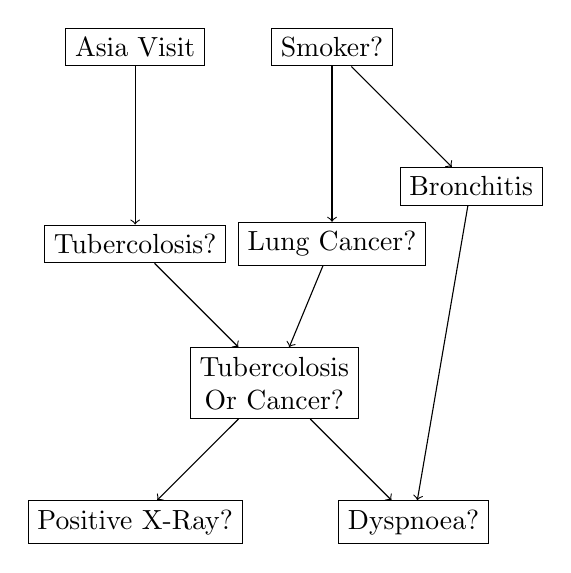
\begin{tikzpicture}[node distance={25mm}, main/.style = {draw, align=center}]
	%% Nodes
	\node[main] (1) {Asia Visit};
	\node[main][right of=1] (2) {Smoker?};

	\node[main][below of=1] (3) {Tubercolosis?};

	\node[main][right of=3] (4) {Lung Cancer?};
	\node[main][below right of=2] (5) {Bronchitis};

	\node[main][below right of=3] (6) {Tubercolosis\\Or Cancer?};          

	\node[main][below left of=6] (7) {Positive X-Ray?};

	\node[main][below right of=6] (8) {Dyspnoea?};     


	%% Edges
	\draw[->] (1) -- (3);
	\draw[->] (2) -- (4);
	\draw[->] (2) -- (5);
	\draw[->] (3) -- (6);     
	\draw[->] (4) -- (6);     
	\draw[->] (6) -- (7);               
	\draw[->] (5) -- (8);
	\draw[->] (6) -- (8);
	\end{tikzpicture}
        \vspace{5mm}
    \caption{Asia Network - Missing Evidence.\\}
  \end{subfigure} \hspace{15mm} 
  \begin{subfigure}[t]{0.4\linewidth} \label{subfig:virtual}
	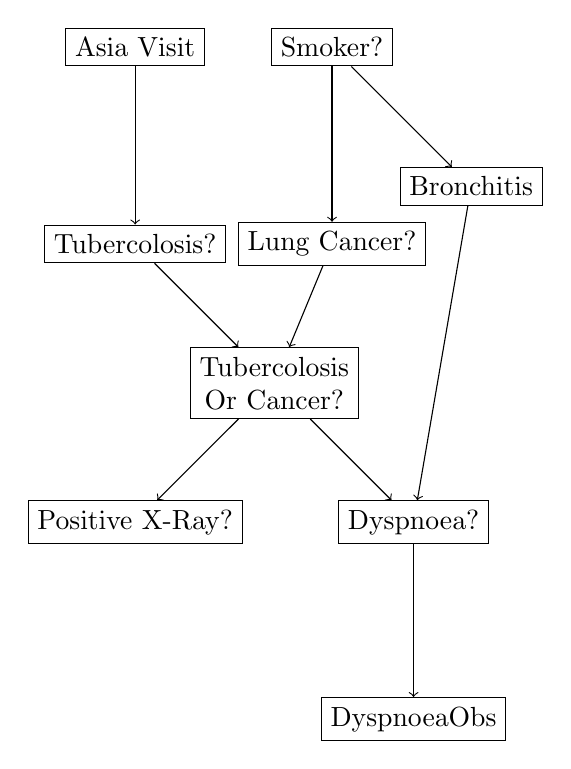
\begin{tikzpicture}[node distance={25mm}, main/.style = {draw, align=center}]
	%% Nodes
	\node[main] (1) {Asia Visit};
	\node[main][right of=1] (2) {Smoker?};

	\node[main][below of=1] (3) {Tubercolosis?};

	\node[main][right of=3] (4) {Lung Cancer?};
	\node[main][below right of=2] (5) {Bronchitis};

	\node[main][below right of=3] (6) {Tubercolosis\\Or Cancer?};          

	\node[main][below left of=6] (7) {Positive X-Ray?};

	\node[main][below right of=6] (8) {Dyspnoea?};     
	\node[draw, distance={10mm}][below of=8] (9) {Dyspnoea \\ Obs};

	%% Edges
	\draw[->] (1) -- (3);
	\draw[->] (2) -- (4);
	\draw[->] (2) -- (5);
	\draw[->] (3) -- (6);     
	\draw[->] (4) -- (6);     
	\draw[->] (6) -- (7);               
	\draw[->] (5) -- (8);
	\draw[->] (6) -- (8);
	\draw[->] (8) -- (9);

	\end{tikzpicture}
        \vspace{5mm}
    \caption{Asia Network - Expanded as by Pearl's Virtual Evidence.}
  \end{subfigure}
  \vspace{0mm}
\end{figure}

Concretely assume as in \cite{Wasserkrug_all} that the ONLP correctly
characterizes Dysponea 70\% of the times when this does in fact
occurs. Note that the ONLP tool does not consider any prior
information resulting from the probabilistic structure of our
network. Then you might encode such likelihood evidence of the ONLP
as in Table \ref{tb:virt-evidence}.

\begin{table}

\begin{center}
\begin{tabular}{|l||*{2}{c|}}\hline
\backslashbox{DysponeaObs}{Dysponea?}
&\makebox[3em]{yes}&\makebox[3em]{no}\\\hline\hline
True & 0.7 & 0.3\\\hline
False & 0.3 & 0.7 \\\hline
\end{tabular}
\end{center}

\caption[Virtual Evidence CPT]{DysponeaObs - Virtual Evidence Node CPT}
\label{tb:virt-evidence}
\end{table}

Given such a CPT, encoding the likelihood evidence, it is possible
to set the DyspnoeaObs to true as a hard finding. In such a way you
will work with a standard network that is just composed of missing
and hard evidence. You can then update the cognitive state of your
network by standard inference techniques, and compute the
parameters of interest by a standard EM-algorithm.

Given such explanation it follows that it is possible to rewrite
the EM-step by adjusting the E-step such that it will perform its
inference step on the virtual evidence augmented network that
respects and incorporates the likelihood evidence information. This
was the intuition and contribution of \cite{Wasserkrug_all} and such
an algorithm, with the corresponding modification of the E-step, is
presented in \ref{alg:EM-Likelihood}.

We continue the next section by modifying such algorithm such that
it is possible to perform MAP estimation in Bayesian settings.


\algrenewcommand\algorithmicindent{1.5em}%

\begin{algorithm*}[h!]
\caption{EM-Likelihood: an EM algorithm for learning with likelihood evidence}
\label{alg:EM-Likelihood}
%\begin{\algsize}
\vspace{-10pt}
\begin{multicols}{2}
\begin{algorithmic}[1] 
\Require Bayesian network $\mathcal{B}=\langle \mathbf{X},\mathbf{D}, G, \mathbf{P} \rangle$, dataset $S$ 

\Procedure{EM}{$\mathcal{B}$, $S$}
\State Initialize $\mathcal{B}$'s parameters $\theta \leftarrow \theta^0$
\ForAll{$t=1, \ldots$ until convergence}
  \State $M-step \ as \ in \ Algorithm \ 1$
\EndFor
\EndProcedure
\\
\Function{Compute-ESS}{$\mathcal{B}=(G,\theta)$, $S$} 

\ForAll {$i\in1,\ldots,n$}
  \ForAll {$x_{i},u_{i}\in Val(X_{i},Pa_{X_{i}}^{\mathcal{B}})$}
   \State $\bar{M}[x_{i},u_{i}]\leftarrow 0$
  \EndFor
\EndFor

% \State (Go over all evidence nodes, creating an augmented network
% for each one, and collect all of the evidence for the nodes in $G$)
\ForAll{example $S_{j}\in S$}

    \State Let $O_j$ be the observations induced by $S_j$
    \State $(G',\theta') \leftarrow$ \textsc{Augment-BN}($\mathcal{B}=(G,\theta)$, $O_{j}$)
    %  (We'll denote $<G',\theta'>$ by $BN_{i}$ as it is the BN induced by example $i$)
    \ForAll{$o \in O_j$}
      \State Set the value of $o_V$ to $true$
    \EndFor
    \State Run inference on $(G',\theta')$ with evidence $d_{j}$
    \ForAll{i$ = 1,\ldots,n$}
      \ForAll{$x_{i},u_{i}\in Val(X_{i},Pa_{X_{i}}^{\mathcal{B}})$}
    
        \State $\bar{M}[x_{i},u_{i}] \mathrel{{+}{=}} P_{(G',\theta')}(x_{i},u_{i}|d_{j})$
    
      \EndFor
    \EndFor
\EndFor
\EndFunction
\\
\Function{Augment-BN}{$\mathcal{B}=(G,\theta)$, $O$} 
  \State Initialize $G'\leftarrow G$, $\theta'\leftarrow\theta$
  \ForAll{$o\in O$}

    \State $G'_{\mathbb{V}}\leftarrow G'_{\mathbb{V}}\cup o_{V}$, $G'_{\mathbb{E}}\leftarrow G'_{\mathbb{E}}\cup(V,o_{V})$      \Comment{Add a new observation node to the graph and connect it to the relevant node}
    \ForAll{$c_{i}\in Conf$}   \Comment{$Conf$ actual likelihood values provided for a node}
      \State $\theta'\leftarrow\theta'\cup\theta_{O_{V}=true|v_{i}}=c_{i}$ \Comment{Set the relevant CPT entry to be $Pr(obs|V=v_{i})$}
    \EndFor
  \EndFor
\State \textbf{return} $(G',\theta')$
\end{algorithmic}
\end{multicols}
%\end{\algsize}
\end{algorithm*}

\newpage

\subsection{Bayesian Learning MAP - Adjusted EM for Likelihood Evidence}
\label{sec:orgc9c2597}

The idea of this section is to extend \ref{alg:EM-Likelihood} in
order to obtain the MAP estimator in a Bayesian Learning setting
with Likelihood Evidence.

We discussed in the previous section how likelihood evidence
requires augmenting the core network by virtual evidence nodes as
in \cite{pearl2014probabilistic} and consequently perform the
inference step on such augmented networks.

Such procedure was outlined by the modification of the E-step in
comparison to the standard EM algorithm with missing evidence.

Moreover we discussed in section \ref{bayes-parameter-learning} we
can adjust the M-step of the EM-algorithm to perform the task of
MAP estimation. Both correctness and convergence properties will
apply such that we will converge to a local maximum for our
posterior distribution.

Combining the two steps it is immediate to see that it is possible
to perform Bayesian Parameter Learning under likelihood evidence
by replacing line 4 of \ref{alg:EM-Likelihood} with 

\begin{algorithm*}[h!]
\caption{Replace M-step for Bayesian Parameter Learning}
\label{alg:Bayes-EM-Likelihood}
%\begin{\algsize}
\vspace{-10pt}
\begin{multicols}{2}
\begin{algorithmic}[1] 
\Require Bayesian network $\mathcal{B}=\langle \mathbf{X},\mathbf{D}, G, \mathbf{P} \rangle$, dataset $S$ 

\Function{M-Step}{$\mathcal{B}$, $S$}
   \State $\theta_{x_{i}|u_{i}}^{t+1}=\frac{\bar{M}_{\theta^{t}}[x_{i},u_{i}] + \alpha_i - 1}{\sum_j \bar{M}_{\theta^{t}}[x_{j},u_{j}] + \alpha_j - 1}$\\
   
   \textbf{return} $(\theta^{t+1})$

\end{algorithmic}
\end{multicols}
%\end{\algsize}
\end{algorithm*}

Given such a computation it is possible to get to a local maximum
for the MAP estimator.

\subsection{Numerical M-step}
\label{sec:org33ae5ff}

This section concludes the chapter on Bayesian Parameter Learning
by substituting the M-step of \ref{alg:Bayes-EM-Likelihood}, by a
numerical estimation of the maximum.

Note, that as argued in the previous sections this has the benefit
of allowing a general algorithm that is not bounded to the
analytical derivation of the maximum in the M-step.

\begin{algorithm*}[h!]
\caption{Replace M-step for Bayesian Parameter Learning}
\label{alg:Numerical-M-Step}
%\begin{\algsize}
\vspace{-10pt}
\begin{multicols}{2}
\begin{algorithmic}[1] 
\Require Bayesian network $\mathcal{B}=\langle \mathbf{X},\mathbf{D}, G, \mathbf{P} \rangle$, dataset $S$, Current Parameterization $\theta_0$, Threshold $\epsilon$

\Function{M-Step}{$\mathcal{B}$, $S$}
   \State Numerically Compute $Q_1$
   \State Numerically Compute $Q_{11}$\\

   \ForAll{$t=0, \ldots$ until convergence}\\
      \State $\theta^{t+1}= \theta_{t} - Q_{11}^{-1} Q_1$\\
      \State convergence if $||\theta^{t+1} - \theta_{t}|| < \epsilon$
   \EndForAll
\end{algorithmic}
\end{multicols}
%\end{\algsize}
\end{algorithm*}


\subsubsection{{\bfseries\sffamily TODO} formulate the things in the paper below}
\label{sec:orgec7b32d}

and incorporate them in the algo above.

\begin{enumerate}
\item {\bfseries\sffamily TODO} define how you compute such numerical derivative.
\label{sec:orga73c0be}

note that you must have the guarantee of positive definite so that
you move towards the maximum despite working with an approximate
numerical term (with error).

this goes together with next section notation. you can then use the
method there in that paper.

wow. so you thought well.


\item {\bfseries\sffamily TODO} note that the above Q terms are nothing else than the expected score and expected fisher information
\label{sec:orgf59eef5}

good paper in \href{https://arxiv.org/pdf/1608.01734.pdf}{this sense}.

\href{https://scholar.google.com/scholar?q=Method\%20for\%20Computation\%20of\%20the\%20Fisher\%20Information\%20Matrix\%20in\%20the\%20Expectation\%2DMaximization\%20Algorithm\&btnG=Search\&as\_sdt=800000000001\&as\_sdtp=on}{other link}.

exactly what I was looking forward to.

incorporate everything in the next step.
\end{enumerate}


\section{On Probabilistic Evidence}
\label{sec:orgbdd7d69}

In the previous chapter we showed how it is possible to rephrase a
likelihood evidence as an observed event by means of augmenting the
network via \emph{virtual evidence}.

We could then propagate the information by means of Bayes Rule
and update the probabilistic structure of the network.

By contrast, with probabilistic evidence such an approach is not
viable. This because, as argued by \cite{PENG_2010}, propagating a
probabilistic finding on \(X \in \textbf{X}\) requires a revision of
the probability distribution of the network P on X by a local
probability distribution defined by the probabilistic evidence
statement R(X). Or, in other words, as in \cite{Mrad_2015}, a
probabilistic finding R(X) requires a reconsideration of the joint
probability distribution P because it replaces the existing prior on
the variable X.

Given the fact that in the presence of probabilistic evidence it is
not possible to propagate evidence in the standard way for the
initial probability, the solution proposed by \cite{jeffrey1990logic},
is to replace the initial probabilistic structure of the network \(P\)
by a new probabilistic structure \(Q\) that reflects the beliefs in
the variables of the model after accepting the probabilistic
evidence.

In the specifics, as well outlined by \cite{Mrad_2015}, according to
what is usually referred as Jeffrey's \emph{probability kinematics}, \(Q\)
must satisfy the following requirements:

\begin{enumerate}
\item the posterior probability distribution on the observed variable X
\(Q(X)\) is unchanged: \(Q(X) = R(X)\). This is in fact the
functional requirement of the probabilistic evidence.

\item the conditional probability distribution of other variables given
\(X\) remains invariant under the observation: \(Q(\textbf{X} \
     {X} | X) = P (\textbf{X} \ {X} | X)\). This essentially means that
even if P and Q disagree on X, they agree on the consequences of
X on other variables \cite{Mrad_2015}.
\end{enumerate}

With the above specification of a new probabilistic structure
satisfying the functional requirements of probabilistic evidence it
is possible to compute the probability of a given event by means of
Jeffrey's rule:

\begin{equation} \label{eq:Jeffreys_Update}
 Q(Z = z) = \sum_x P(Z = z | X = x) R(X = x)
\end{equation}

Note that Jeffrey's formula above \ref{eq:Jeffreys_Update}, albeit
being theoretically compelling, cannot be directly applied in
Bayesian Networks, as it requires the specification and functional
form of the full probabilistic structure of the network in any state
of the network in order to compute P(Z = z | X = x). This must be
computed according to some inference step.

The solution to this problem as suggested by \cite{Chan_2005} and
\cite{PENG_2010} is to frame probabilistic evidence into likelihood
evidence by computing the likelihood ratio as defined by:

\begin{align} \label{eq:probabilistic-to-likelihood-evidence}
 L(X) = (\frac{R(x_1)}{P(x_1)}: ... : \frac{R(x_k)}{P(x_k)})
\end{align}

It is then possible to prove that propagating such likelihood
evidence by means of Pearl's method as described in the previous
section, is equivalent to propagating and obtain the probabilistic
structure by means of Jeffrey's method \ref{eq:Jeffreys_Update}.

It is in fact possible to prove, as in \cite{PENG_2010}, that with
such an approach the posterior probability of X after propagating
L(X) by Pearl’s method, is equal to R(X).

Given such theory it is straightforward to understand that
in the case of a single probabilistic evidence we can easily learn
the parameters of the Bayesian Network via the following adjustment
of the \textbf{AUGMENT-BN} function of \ref{alg:EM-Likelihood}

\algrenewcommand\algorithmicindent{1.5em}%

\begin{algorithm*}[h!]
\caption{EM-Likelihood: an EM algorithm for learning with likelihood evidence}
\label{alg:EM-Likelihood}
%\begin{\algsize}
\vspace{-10pt}
\begin{multicols}{2}
\begin{algorithmic}[1] 
\Require Bayesian network $\mathcal{B}=\langle \mathbf{X},\mathbf{D}, G, \mathbf{P} \rangle$, dataset $S$, Observations $O$

\Function{Augment-BN}{$\mathcal{B}=(G,\theta)$, $O$} 
  \State Initialize $G'\leftarrow G$, $\theta'\leftarrow\theta$, $Conf \leftarrow \emptyset$
  \ForAll{$r_i\in ProbEv(x_j)$}  \Comment{$ProbEv$ is the passed probabilistic evidence. r are the states for the Node.}
    $Conf \leftarrow \frac{r_i}{\mathbf{P}_{x_j}}$ 
  \EndFor
  \ForAll{$o\in O$}
    \State $G'_{\mathbb{V}}\leftarrow G'_{\mathbb{V}}\cup o_{V}$, $G'_{\mathbb{E}}\leftarrow G'_{\mathbb{E}}\cup(V,o_{V})$      \Comment{Add a new observation node to the graph and connect it to the relevant node}
    \ForAll{$c_{i}\in Conf$}   \Comment{$Conf$ computed likelihood for a probabilistic node}
      \State $\theta'\leftarrow\theta'\cup\theta_{O_{V}=true|v_{i}}=c_{i}$ \Comment{Set the relevant CPT entry to be $Pr(obs|V=v_{i})$}
    \EndFor
  \EndFor
\State \textbf{return} $(G',\theta')$
\end{algorithmic}
\end{multicols}
%\end{\algsize}
\end{algorithm*}

This concludes the section. It is important to mention, to this
point that in the case of multiple probabilistic evidence on
different nodes, the above approach does not apply.

This because, as shown by example, by \cite{PENG_2010}, the algorithm
above is not commutative and does not guarantee - for instance for
the case R1(X1) and R2(X2) - \(Q(X1) \neq R1(X1)\) or \(Q(X2) \neq
   R(X2)\), depending on the order of propagation.

In order to solve such an issue, and guarantee the functional
requirement of probabilistic evidence, a method was proposed by
\cite{PENG_2010}. This involves the combination of an \emph{Iterative
Proportional Fitting Procedure (IPFP) algorithm} with the \emph{big
clique algorithm}. Nonetheless, we leave it as a further avenue of
research to extend such methods in order Bayesian Parameter
Learning.

\newpage


\section{TODOs}
\label{sec:org256cb5c}

\begin{enumerate}
\item {\bfseries\sffamily TODO} check if particle formulation in energy functional ok as such
\label{sec:orgcdf22a4}

\item {\bfseries\sffamily TODO} note that network structure G(V,X) how you described. Correct later
\label{sec:orgfa08069}

\item {\bfseries\sffamily TODO} make more explicit the citation to koller and friedman in the chapter about the mathematics of the EM algo
\label{sec:org58af0b2}

\item {\bfseries\sffamily TODO} make more explicit the difference between synthetically completed missing observations and <?>
\label{sec:orgbf03418}

\item {\bfseries\sffamily TODO} note that the EM you loose global decomposition such that at the end with the local maxima of CPDs achieved by EM you ultimately just get a local maximum.
\label{sec:orgb8f49ad}

\newpage

\bibliography{../literature/references}
\bibliographystyle{unsrt}




\item {\bfseries\sffamily TODO} for last section - check at the following chapter.
\label{sec:org3a92251}

Concept: Representation Independence - in chapter 17 of the
koller book. this is central as if that breaks apart the entire
modeling and parameterization and models outlined here in the
thesis fall apart.

you should therefore be careful with it.

\item {\bfseries\sffamily TODO} check chapter 17 for making the point below
\label{sec:org4a81251}

say at the end that the entire theory does not hold for locally
shared and globally shared network parameters. there you would
have to adjust the entire thing
\end{enumerate}
\end{document}
